% Chapter 4

\chapter{Technical Details} % Write in your own chapter title
\label{Chapter4}
\lhead{Chapter 4. \emph{Technical Details}} % Write in your own chapter title to set the page header

%\begin{wraptable}[]{r}{0.45\textwidth}
  %\caption{Lines of code for Polly, SPolly and Sambamba components}
  %\begin{center}
    %\begin{tabular}{ l r }
     %component     & LOC  \\
      %\hline
      %SPolly     & XXX \\
      %~ Region Speculation     & 2045 \\
      %~ SPolly Sambamba CT  & 102 \\
      %~ SPolly Sambamba RT  & XXX \\
      %Polly     & 12643 \\
      %~ SCoP Detection     & 604 \\
      %~ Code Generation    & 1793 \\
      %Sambamba     & 23533 \\
      %~ Profiler   & 269 \\
      %~ Statistics   & 85 \\
    %\end{tabular}
  %\end{center}
  %\label{tab:LinesOfCode}
%\end{wraptable}

SPolly in its entirety is a compound of three parts. The region speculation, 
embedded into Polly, and the two Sambamba modules  for compile time and
runtime respectively. The region speculation part is the interface
to all discovered sSCoPs, thus it contains most of the transformation code, 
while the Sambamba passes concentrate on the program logic. 
At the moment the runtime part is far more evolved and the compile time component
plays only a minor role. Apart from SPolly itself, a basic profiler and a
statistic module for Sambamba arose during this work. Both have been very helpful
during the development and may become permanent features of Sambamba.

%During the implementation various bugs occurred and even if most of them
%arose by my own fault I triggered some in the code base of Polly and 
%Sambamba too. A full list of reported bugs is given in Table 
%\ref{tab:Bugreports}. 

%Table \ref{tab:LinesOfCode} compares the work in a
%quantitative manner as it lists the lines of code (LOC) added for SPolly as well
%as for Sambamba and Polly parts. The 

%[TODO rephrase] 
%Table \ref{tab:CommandLineOptions} lists all available command line options 
%added in the context of SPolly. Although all of these options work 
%without the Sambamba modules, yet Sambamba at all, the last three would only 
%produce sequential executable code without any parallelization. 
%[TODO] As for now I am not quite sure if this could be of any practical use, 
%but to my understanding Polly could get a similar option in the near future. 


\section{SPolly in a Nutshell}
%SPolly, as presented here, is composed of a compile time and a runtime part. 
%Their respective tasks are related but not the same. During both steps the, so
%called, region speculation is used to interact with Polly. 
%It is also the 
%part of SPolly which is not integrated  into the Sambamba framework. As some
%of the functionalities do not rely on speculation, it is possible to integrate
%them into the main application of Polly anytime soon. 

%\paragraph{Compile Time }~\\
\begin{wrapfigure}[]{r}{0.4\textwidth}
  \centering
  %\vspace*{-4mm}
  \includegraphics[width=0.4\textwidth]{Figures/draftPaperCT.eps}
  \caption{Draft paper: \\SPolly at compile time}
  \vspace*{-4mm}
  \label{fig:draftPaperCT}  
\end{wrapfigure}
During \textbf{compile time} the main goal of SPolly is to simplify the runtime part,
by reducing runtime overhead through preprocessing and even static method versioning.
First the SCoP detection tries to find all valid regions within the given LLVM-IR
(according to the SCoP definition; Table \ref{tab:SCoPRestrictions}).
But instead of rejecting a region once a restriction is violated, 
the region speculation is asked how to proceed. Rejection causes we want to speculate
on namely aliasing, non-affine base pointers and function calls, 
are gathered by the region speculation, but fully transparent to the SCoP detection.
This proceeding allows to find all violations within a region and to treat valid and
speculatively valid ones nearly the same. After all  
speculatively valid SCoPs are encountered the Sambamba compile 
time part takes action. It separates the sSCoPs as some of them do not need
speculation at all. Those sSCoPs are optimized and exchanged, 
while the others are currently only extracted. This means they are replaced by
calls to functions only containing the speculatively valid region. 
%(see \ref{RegionExtraction}).
At the moment, no pre computation takes place and only sSCoPs with complete
alias tests are considered to be optimized and exchanged immediately.  Future 
work on SPolly could change this in order to reduce the workload during runtime.

%Further details on
%the ratings are given in section \ref{RegionScores} while 
%section \ref{SpeculationFreesSCoPs} coveres the case of speculation free sSCoPs.




%\paragraph{Runtime }~\\
\begin{wrapfigure}[]{l}{0.5\textwidth}
  \centering
  \vspace*{-4mm}
  \includegraphics[width=0.5\textwidth]{Figures/draftPaperRT.eps}
  \caption{Draft paper: \\ SPolly at runtime}
  \vspace*{-2mm}
  \label{fig:draftPaperCT}  
\end{wrapfigure}
The \textbf{runtime} part of SPolly first retrieves the extracted sSCoPs and 
precomputed versions from the data store. If not already done during  compile
time, profiling versions will be created. It would be possible to restrict
this to the highest rated sSCoPs only, but as the creation is cheap, only 
a few additional instructions without traversing the code again, and the execution 
overhead for most of them is non-existent it is feasible to do so for rather bad
ranked sSCoPs as well.  Those profiling versions will now collect information
not only about the time consumption of the sSCoP, but also about loop bounds,
branch probabilities and the results of introduced checks. Except for the time
consumption these values will affect the rating of the sSCoP which again is used
to identify promising sSCoPs.

%The next section will explain this rating and the effects of profiling in more 
%detail, while section \ref{IntroducedTests} covers the test creation and theirs use. 
%As explained above, the combined static and dynamic information determine which region
%is promising, thus which region will be speculatively optimized and in the end
%executed in parallel.






\section{Speculative Polly}
You could look at SPolly as extension to Polly, especially designed
to interact with Sambamba. As such it was crucial to preserve all functionality 
of Polly and supplement it with new ones. Most of them are
implemented in the region speculation, but there are some new options in the 
code generation too. Pollys SCoP detection was chosen to serve as a
bridge between Polly and the speculative part as speculative valid regions 
would be rejected here. The information currently needed for region speculation
is also available at this point and can be directly reused. 

As the architecture of Polly was nicely illustrated in the thesis of Tobias 
Grosser\cite{grosser:thesis}, we extended the Figure to capture the changes 
introduced by SPolly, too (see Figure \ref{fig:SPollyArchitecture}). 
In comparison to the original one, the region speculation, 
the unrolling backend and the splitting backend have been added. 

\clearpage
~\\
\begin{figure}[htbp]
  \centering
  \includegraphics[width=0.85\textwidth]{SPollyArchitecture.eps}
  \caption{SPolly - The Architecture ~\\ (Based on ``Polly - The Architecture''\cite{grosser:thesis})}
  \label{fig:SPollyArchitecture}  
\end{figure}
~\\


\subsection{Region Speculation}
The region speculation  of SPolly has several tasks to fulfill. The first 
one includes the communication with Polly or, to be more precise, 
with the SCoP detection. Each region analyzed by the SCoP detection needs to be
considered as possibly speculatively valid SCoP, thus
all information exposed during the detection is stored.
If the region contains a sSCoP violation, 
listed in Table \ref{tab:sSCoPRestrictions}, or if it is without any validation,
the information is discarded. In the latter case, the region is a valid 
SCoP and will be handled by Polly and in the former one it is neither a SCoP nor 
an sSCoP, hence we cannot optimize it any further.
For all others regions a new sSCoP is created and initially validated. 
This validation mainly computes information needed for later
transformations but it may discard the sSCoP too. This is the case if 
violating function calls, e.g., a \texttt{printf}, occur on every execution path.
As the \textit{Concept} Chapter described how to handle such cases in general,
we may include even those in later work. For now, violating calls
are only allowed in conditionals as such cases provide much more speculation
potential. \\
%Despite the fact that both, rarely as well as always executed calls,
%cannot be secured by the current STM implementation, we believe that the 
%region score heuristic only suggests sSCoPs with high speculative potential and
%low chance of misspeculation.  \\

\begin{table}[htbp]
\begin{framed}
  \centering
  \caption{Restrictions on sSCoPs}
    \begin{itemize}
      \renewcommand{\labelitemi}{$\triangleright$}
      \item Only simple regions not containing the entry block of the function
      \item Only nested loops and conditionals
      \item Only branches with affine conditions
      \item No unsigned iteration variables
      \item Only canonical PHI nodes and induction variables
      \item No alloca or cast instructions within the region
      \item Only affine trip counts for loops
      \item Only guarded ``violating'' function calls
      \item No PHI nodes in the region exit block
      \item \textit{At least one loop contained}
    \end{itemize}
    %\flushleft{\footnotemark[2] open for future work of SPolly}
  \label{tab:sSCoPConstraints}
  \label{tab:sSCoPRestrictions}
  \label{sSCoPRestrictionsPage}
\end{framed}
\end{table}

\subsection{Region Scores}
Initial efforts to create region scores in order to rank sSCoPs 
did not use any kind of memory, 
thus the whole region was analyzed every time new information was available.
To avoid these unnecessary computations the current score is a
symbolic value which may contain variables for values not known statically, e.g.,
branch probabilities or loop bounds.
Evaluation of these symbolic values will take all profiling 
information into account and yield a comparable integer value. 
Only during the initial creation of the score expression the region needs to be
traversed to find all used parameters and branches. 


\subsection{sSCoP Extraction}
\label{sSCoPExtraction}
The sSCoP extraction was designed to simplify the method versioning for functions 
containing several speculatively valid SCoPs. It creates a new sub function for 
every sSCoP and inserts a call in the respective place. On the one hand the creation 
of profiling and parallel versions as well the later function exchanging becomes
a lot easier and cheaper this way. On the other hand it is the first step to 
multiple specialized versions, e.g., with constant instead of variable loop 
bounds. Another possible benefit of this strategy is that the transformations 
applied to an sSCoP (or SCoP) would not affect other code regions anymore. 
%In rarely occurring cases Polly rejects regions because transformations could
%break outer constraints. 



%\subsubsection{Method Versioning}
%Method versioning is one of the great benefits of the Sambamba system and allows
%to adapt the execution at runtime. In the scope of this work two different 
%versions are created, a profiling one and an optimized one. 
%Up to this point several suggestions for other possible, mainly specialized, 
%versions have been mentioned (e.g., with constant instead of variable parameters or 
%optimized with different tile sizes). 
%Most of them would benefit from the SPolly infrastructure as 
%profiling data is available and the extracted sSCoPs simplify cloning and
%transformations. A full list of feasible versions as well as detailed thoughts 
%on them is presented in the future work section of the last chapter.


%\paragraph{The Profiling Version}
%~\\
%Profiling is a powerful ability for just in time compiled programs, like the ones
%produced by Sambamba. SPolly benefits not only from the introduced tests, but also
%from the monitored branch probabilities and loop trip counts. The retrieved 
%information are in the first place used to compute the region scores, thus to
%improve the heuristic which chooses sSCoPs for optimization. Later on,
%this information could help other analyses and transformations too.


%\paragraph{The Optimized Version }
%~\\
%Optimized versions are in the first place those sSCoPs which have been 
%optimized by Polly and parallelized by either Polly or Sambamba. As SPolly is  
%currently not applying only optimizations without parallelization there is no
%need to speak of parallelized versions explicitly. At the moment it is also true
%that all sSCoPs chosen for optimization are feed into Polly. Even though Polly 
%might not be able to apply transformations, 
%it will certainly create the CFG structure already presented in 
%figure \ref{fig:PollyCFG}. This proceeding is beneficial on two 
%accounts. First it allows to reuse the Polly code generation which creates a  
%normalized loop structure and nowadays also one of two easy parallelizable 
%outer loop shapes (see next section for more details). The second benefit 
%concerns the new CFG in its entirety. Tests, like the already implemented alias
%test, can be easily placed in front of a speculatively optimized loop. 
%Technically it is very similar to a runtime dispatcher which chooses between,
%at the moment, two available versions. As this structure is always given, the
%default behaviour of SPolly is to introduce as many alias tests as possible 
%when a optimized version is created. Different additional tests or versions 
%could use this structure as they would only need to modify the split block in front
%of the sequential and parallel version. 



\subsection{Code Generation}
\label{CodeGeneration}
As part of the extension of Polly two new code generation backends were added. 
Apart from sequential, vectorized and OpenMP code generation, SPolly is 
capable of creating easily parallelizable loop shapes with regard to fork-join
parallelism. The first one is an unrolled and blocked loop as denoted by the 
translation from Figure \ref{lst:ForkJoinCodeGenerationSRC} to
Figure \ref{lst:ForkJoinCodeGenerationOUT}. A parallel version of this loop will
execute the N blocked and unrolled iterations concurrently, while there might 
be remaining ones which are executed sequentially after the loop. 
Figure \ref{lst:ForkJoinCodeGenerationSPLIT} shows the outcome if the other new
backend is used. This time the whole loop nest was fragmented into N ``identical''
ones but with adjusted loop bounds. The main difference between these two approaches 
is the workload per transaction. While the former one will only execute one
loop iteration at a time, the latter one will execute one N-th of the 
iteration space (for N $\ll$ loop trip count). The main similarity is the
simple CFG structure, which is easily convertible to a ParCFG.
Figure \ref{fig:CreateParCFG} and \ref{fig:CreateParCFG2} illustrates such
transformations for the blocking backend and the splitting backend respectively.  

Since STM transactions will always cause synchronization overhead,
the second approach has certain advantages over the first one; e.g., 
if N is chosen as the number of available threads, the overhead is minimal, 
compared to the achieved parallelism. This is the ``best case'' as long as no
misspeculation takes place. If there are speculatively removed dependencies
the former approach might perform better, but in the extrem case where all iterations
depend on former ones, the second one has an advantage again. As this holds only
in theory, Section \ref{Rollbacks} compares the maximal number of rollbacks 
for both new code generation backends in more detail. 
%It also shows that it is not yet clear 
%which one will do better under different circumstances,
%hence there are situations 

%translated into an ParCFG, thus parallelized by a Sambamba module. Listing 
%\ref{lst:ForkJoinCodeGenerationOUT} presents this transformation. The special 
%case where lower and upper bound as well as the 
%stride are statically known constants, the second loop, which computes 
%remaining iterations, is completely unrolled.
%This kind of loop unrolling and blocking may find its 
%way into Polly in the near future. 



%\subsubsection*{Parallelization}
%In order to secure the speculative executions with Sambambas STM
%(see \ref{SambambaSTM}) the Sambamba parallelizer needs to be used.
%As this parallelizer does not yet support loop parallelization per se, some 
%transformation needed to be done first. The new code generation type was created
%to do the difficult one without recomputing information provided during by the
%polytope model (during the code generation) anyway. As these transformation
%yields code as in listing \ref{lst:ForkJoinCodeGenerationOUT} the creation of
%a ParCFG (see \ref{SambambaParCFG}) remains. Figures \ref{fig:ForkJoinCFG} and
%\ref{fig:ForkJoinParCFG} visualize these changes.


\lstset{frame=none}
\begin{figure}[htbp]
  \centering
  \subfloat[Initial loop nest]{
    \begin{minipage}[c][0.7\width]{0.45\textwidth}
    \lstinputlisting{Primitives/Code/ForkJoinCodeGenerationSRC.c}
    \label{lst:ForkJoinCodeGenerationSRC}
    \end{minipage}
  }
  \subfloat[Figure \ref{lst:ForkJoinCodeGenerationSRC} after N iterations have been blocked and unrolled (Unrolling backend)]{
    \begin{minipage}[c][0.7\width]{0.45\textwidth}
    \lstinputlisting{Primitives/Code/ForkJoinCodeGenerationOUT.c}
    \label{lst:ForkJoinCodeGenerationOUT}
    \end{minipage}
  }

  \subfloat[Figure \ref{lst:ForkJoinCodeGenerationSRC} after loop splitting (Splitting backend)]{
    \begin{tabular}{c}
      \lstinputlisting{Primitives/Code/ForkJoinCodeGenerationSPLIT.c} \\
      \label{lst:ForkJoinCodeGenerationSPLIT}
    \end{tabular}
  }
  \caption{Outcome of the new code generation backends}
\end{figure}

\begin{figure}[htbp]
  \centering
  \subfloat[CFG after blocking and unrolling]{
  \centering
    \begin{minipage}[c][7cm]{0.5\textwidth}
    \centering
      \begin{tabular}{c}
    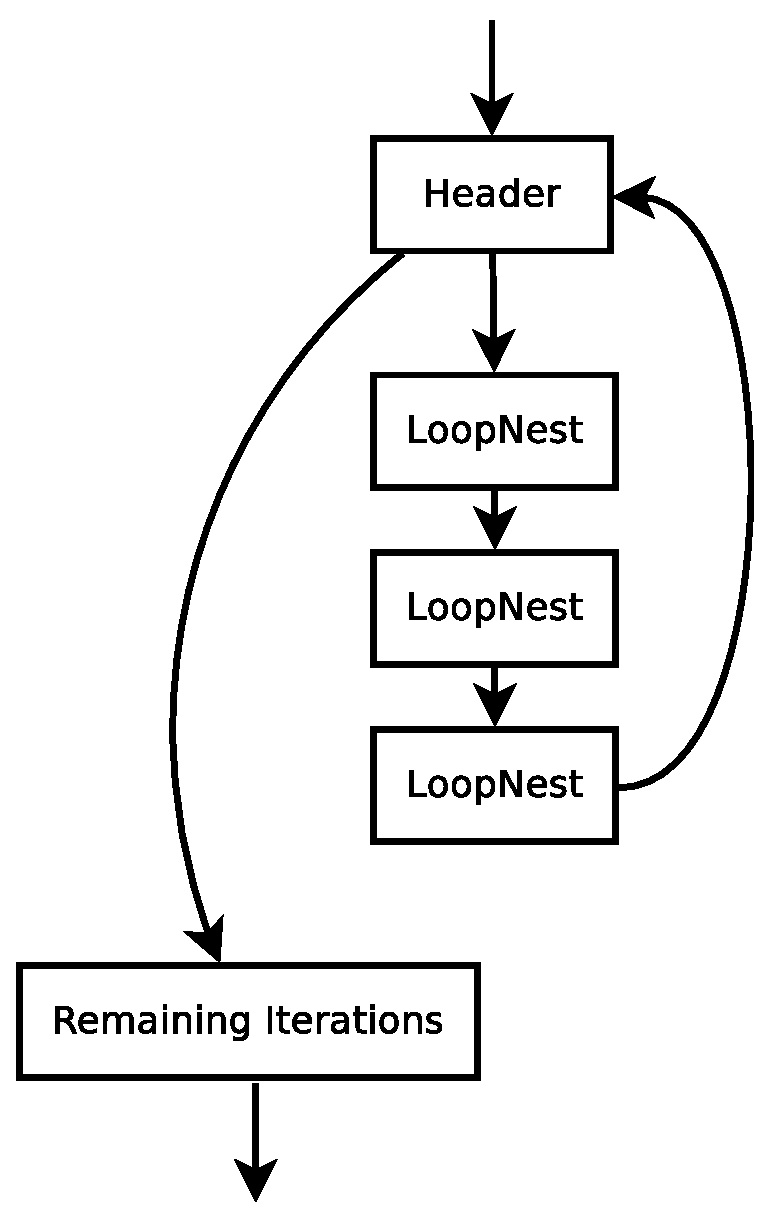
\includegraphics[height=6cm]{Figures/ForkJoinCFG.eps}
    \label{fig:ForkJoinCFG} 
  \end{tabular}
    \end{minipage}
  }
  \subfloat[ParCFG created from Figure \ref{fig:ForkJoinCFG}]{
  \centering
    \begin{minipage}[c][7cm]{0.5\textwidth}
    \centering
      \begin{tabular}{c}
    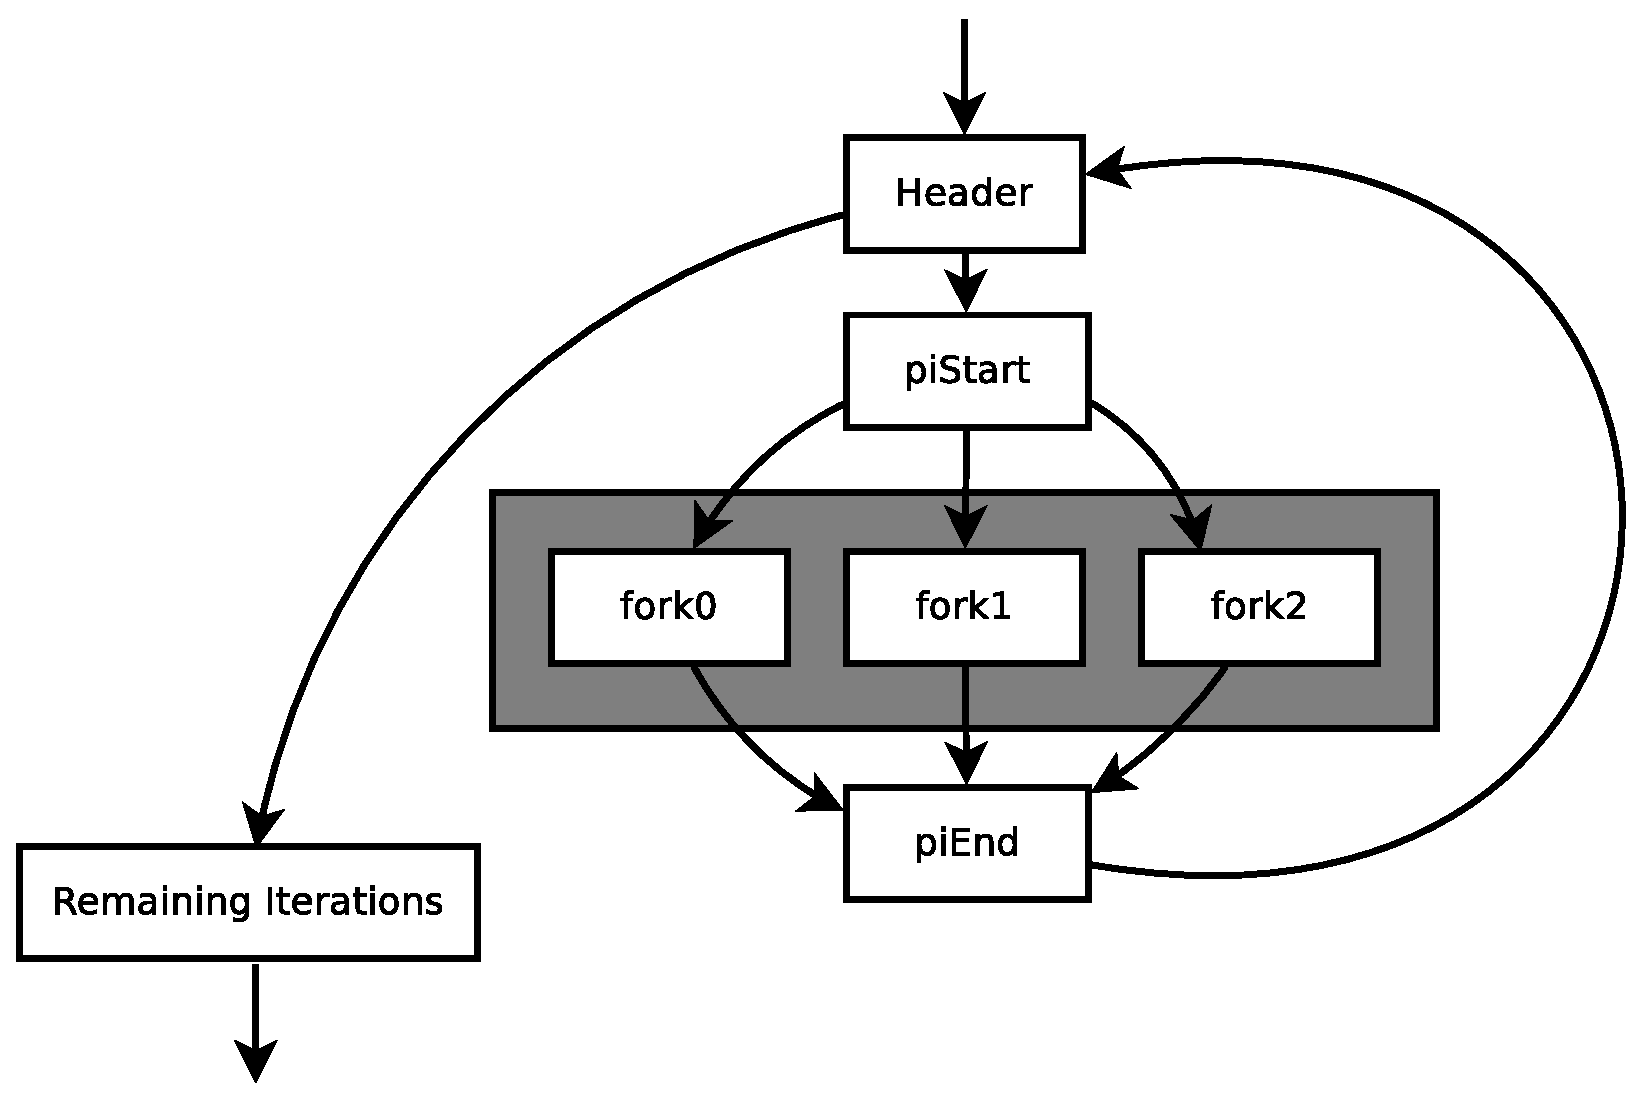
\includegraphics[height=6cm]{Figures/ForkJoinParCFG.eps}
    \label{fig:ForkJoinParCFG}
  \end{tabular}
    \end{minipage}
  }
  \caption{Forked (Par)CFG after the blocking backend was used}
  \label{fig:CreateParCFG}  
\end{figure}

\begin{figure}[htbp]
  \centering
  \subfloat[CFG after loop splitting]{
    \begin{minipage}[c][7cm]{0.5\textwidth}
    \centering
      \begin{tabular}{c}
    \includegraphics[height=6cm]{Figures/ForkJoinCFG2.eps}
    \label{fig:ForkJoinCFG2} 
  \end{tabular}
    \end{minipage}
  }
  \subfloat[ParCFG created from Figure \ref{fig:ForkJoinCFG2}]{
    \begin{minipage}[c][7cm]{0.5\textwidth}
    \centering
      \begin{tabular}{c}
    \includegraphics[height=6cm]{Figures/ForkJoinParCFG2.eps}
    \label{fig:ForkJoinParCFG2}
  \end{tabular}
    \end{minipage}
  }
  \caption{Forked (Par)CFG after the splitting backend was used}
  \label{fig:CreateParCFG2}  
\end{figure}
\resetlst

%\section{Sambamba Compile Time Module}
%The compile time part of the Sambamba module locates all sSCoPs
%within the given input. Those sSCoPs are extracted if the applicable tests are 
%not complete. All extracted sSCoPs are stored within the created Sambamba 
%bitcode or respectively executable file. Extracting every single sSCoP 
%decreases the performance as it introduced new call instructions, 
%but it also allows to easily change and combine different optimized sSCoPs, 
%even if they originated from the same function.   
%The functionality of the compile time part is minimal but it helps to focus 
%on profiling and execution during runtime. 
%Further work could heavily improve this part, beginning by compile time 
%preparation of the sSCoPs, up to precomputed profiling and optimized versions.



%\section{Sambamba Runtime Module}

%In addition to the compile time parts, which only rely on static analyses,
%the runtime part uses different kinds of runtime information to decide. 
%To take advantage of this extra knowledge, most of the decisions, thus most of
%the program logic, is implemented in the runtime module. 


%Table \ref{}[TODO] gives an overview of the functionalities.


%\begin{table}[htbp]
  %\caption{Functionality of the SPolly Sambamba module}
  %\begin{tabular}{| l |}
    %\hline
    
    %\hline
    %\hline

    %\hline
  %\end{tabular}
%\end{table}



\section{Profiling for Sambamba}

Sambamba, as research project under heavy development, was not capable of any kind
of profiling at the beginning of this work. 
By now, there are two profilers available.
The first one, implemented by the authors of Sambamba, 
is used for exact time measuring, while the other one was created considering
the needs of SPolly. It is capable of collecting execution counts for arbitrary
program locations and offers an interface to measure and compute
branch probabilities as well as loop trip counts. Apart from profiling executions
it can also be used to monitor variables at given program locations, useful 
in the context of specialization as it might
provide hints on ``quasi constant'' parameters. If such parameters are encountered,
specialized versions may yield additional speedups. 




% ID | description | status | patch included | tool
\begin{table}[htbp]
\begin{framed}
  %\vspace*{10mm}
  \centering
  \caption{Reported bugs}
  \begin{tabularx}{\textwidth}{ c | X | c | c | c }
   Bug-ID & Description & Status & Patch provided  & Component \\
  \hline \hline
  12426 & Wrong argument mapping in OpenMP subfunctions & FIXED & partially & Polly \\
   \hline
  12427 & Invariant instruction use in OpenMP subfunctions & NEW & yes & Polly \\
   \hline
  12428 & Wrong PHInode use in OpenMP subfunctions & NEW & no & Polly \\
   \hline
    N/A & Wrong computations of STM guarded code & FIXED & no & Sambamba \\
  \end{tabularx}
  \label{tab:Bugreports}
\end{framed}
\end{table}



